\section{Введение. Аксиоматика}

Для дальнейшей работы договоримся об основных понятиях.\\

\begin{enumerate}
    \item Мы работаем в евклидовом пространстве $E^3$.
    \item Скалярным параметром является время t. В основном, хоть аксиоматика этого и не требует, будем считать, что время монотонно и непрерывно.
    \item \textbf{Система отсчета} --- это некоторый базис $(\vec{e_1}, \vec{e_2}, \vec{e_3})$ в $E^3$ и выбор параметризации.
    \item Основным объектом исследования является \textbf{материальная точка} $\{\vec{r}, m\}$, где $\vec{r}$ --- радиус-вектор, а $m$ --- масса, считаем, что $m = const$.
    \item \textbf{Движение} --- это отображение из $R'$ в $E^3$ или зависимость положения точки в данном базисе от времени. При этом:
    \begin{itemize}
        \item $\vec{r}(t)$ --- \textbf{закон движения}
        \item $\vec{v} = \dot{\vec{r}}(t)$ --- \textbf{скорость}
        \item $\vec{w} = \ddot{\vec{r}}(t)$ --- \textbf{ускорение}
    \end{itemize}
    \item Будем говорить, что пара материальных точек \textbf{взаимодействует}, если с ними ассоциированы силы $\vec{F_1}$ и $\vec{F_2}$ такие, что $\vec{F_1} = -\vec{F_2}$, коллинеарные $\vec{r_1} - \vec{r_2}$, т.е. прямой, соединяющей эти точки в пространстве. Это III закон Ньютона.
    \item Существует система отсчета (инерциальная) такая, что для любой материальной точки выполнен II закон Ньютона, т.е.
    \[
    m\ddot{\vec{r}} = \vec{F}
    \]
\end{enumerate}

На самом деле, большинство систем не являются инерциальными, но с некоторыми приближениями мы можем считать их таковыми. Примером такой квази-инерциальной системы является система отсчета, начало которой связанно с центром Земли, а оси движутся поступательно. Начало системы отсчёта не покоится и не движется прямолинейно и равномерно, несмотря на это такая система рассматривается в качестве инерциального базиса во многих задачах астродинамики/баллистики при изучении движения искусственных спутников Земли.

\begin{theorem}[Принцип Галилея]
При переходе от одной ИСО с некоторым базисом $\mathcal{E}$ и временем t к другой системе отсчета с базисом $\mathcal{E}'$ и временем $t'$ с помощью преобразований
\[
    \vec{r'} = \vec{v_0}t + \vec{r_0} + A\vec{r}, \tab t' = t + \tau,
\]
получим ИСО. Здесь $A$ --- ортогональная матрица, задающая взаимную ориентацию базисов, $\vec{r_0}$ --- вектор, соединяющий начала отсчета в двух базисах в начальный момент времени, $\vec{v_0}$ --- относительная скорость базисов, $\tau$ --- разность начала отсчета времени в разных базисах.
    
\end{theorem}

Заметим, что свойство \textit{инвариантности} уравнений не тоже самое, что и инвариантность правила составления этих уравнений, называемая \textit{ковариантностью}. В частности, уравнения Ньютона ковариантны относительно приведенных выше преобразований.\\

Также заметим, что мы нигде не упоминали I закон Ньютона, но в этом и нет необходимости, т.к. он очевидным образом следует из аксиом.





\section{Кинематика}

\subsection{Кинематика материальной точки}

Возьмем ПДСК в $E^3$.

\begin{wrapfigure}{}{0.5\textwidth}
	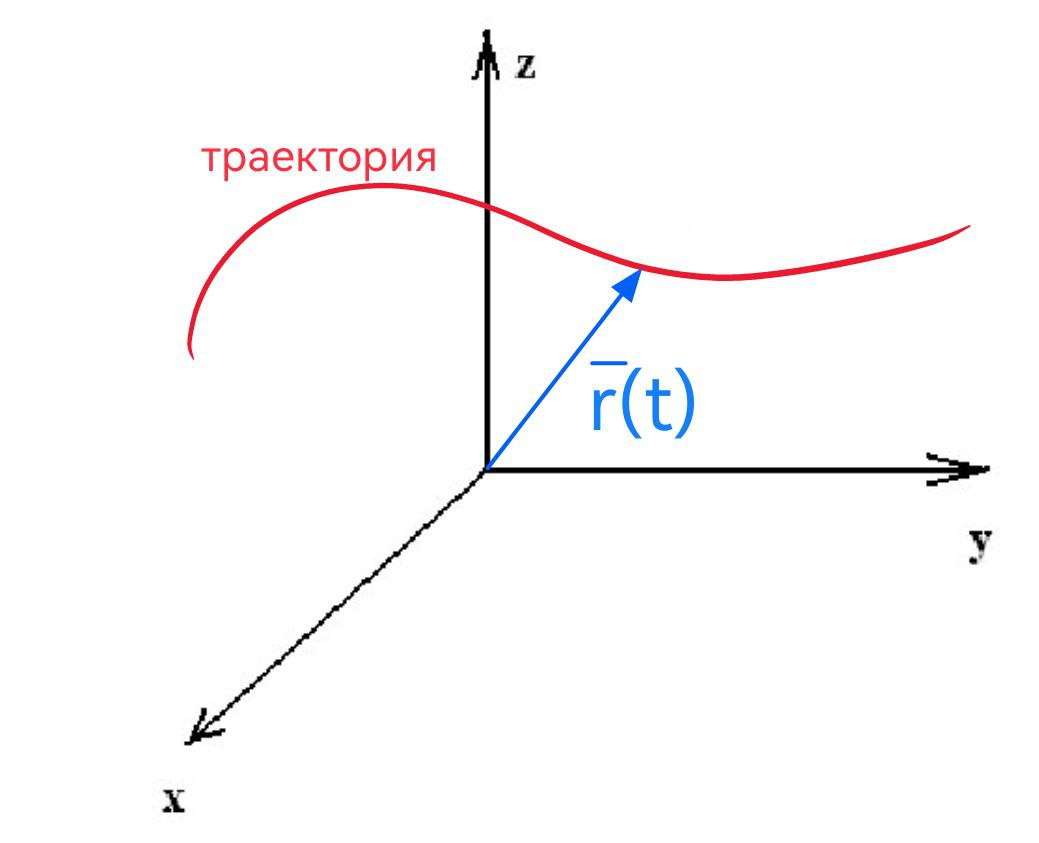
\includegraphics[width=0.8\linewidth]{images/лекция_1_1.jpeg}
\end{wrapfigure}

	\[
    \vec{r}(t) = \begin{pmatrix*}
        x(t)\\
        y(t)\\
        z(t)\\
    \end{pmatrix*}, \tab
    \vec{v} = \dot{\vec{r}}(t) = \dfrac{d\vec{r}(s)}{ds} \cdot \dfrac{ds}{dt} = v \cdot \vec{\tau},
    \]

    где $\dfrac{d\vec{r}(s)}{ds}$ --- вектор касательной, а $\dfrac{ds}{dt}$ --- модуль скорости.



\begin{wrapfigure}{l}{0.5\textwidth}
	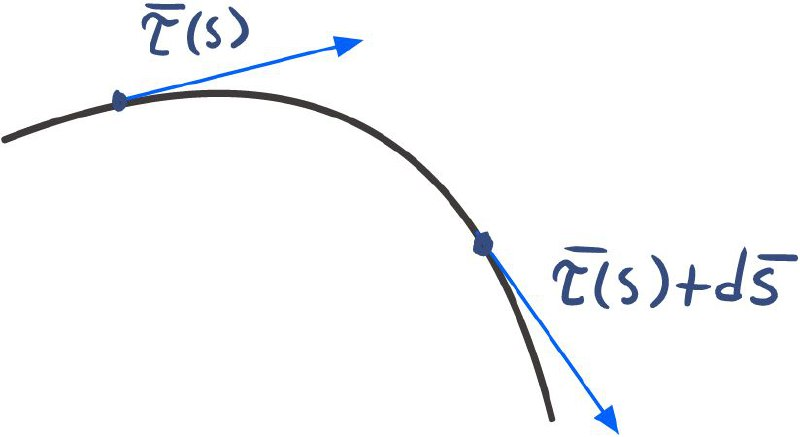
\includegraphics[width=0.8\linewidth]{images/лекция_1_2.jpeg}
\end{wrapfigure}
\tab\\ \tab\\ \tab\\ \tab\\
Получили, что скорость направлена по касательной к траектории точки.\\

Производная вектора, которая не меняется по модулю, перпендикулярна ему.

\[
\vec{w} = \dot{\vec{v}} = \dot{v}\vec{\tau} + v\dot{\vec{\tau}}
\]

Заметим, что $\dot{\tau}$ можно переписать в виде $\dot{\tau} = \dfrac{d \vec{\tau}}{d s}\dfrac{d s}{d t}$, где $\dfrac{d s}{d t}$ --- модуль скорости, а $\dfrac{d\vec{\tau}}{d s} = \dfrac{1}{\rho}\vec{n}$ --- \textit{вектор кривизны}, а $\rho$ --- \textit{радиус кривизны} траектории в данной точке. Подставив в уравнение для ускорения, получим

\begin{equation}
    \vec{w} = \dot{v}\vec{\tau} + \dfrac{v^2}{\rho}\vec{n} = \vec{w_{\tau}} + \vec{w_n}
\end{equation}

Здесь $\vec{w_{\tau}}$ --- \textit{тангенциальное}, а $\vec{w_n}$ --- нормальное ускорения.

\begin{definition}
    Правая тройка попарно ортогональных векторов $(\vec{\tau},~\vec{n},~\vec{b)}$ называется \textit{естественным трехгранником}.
\end{definition}
\newpage
\begin{wrapfigure}{l}{0.5\textwidth}
	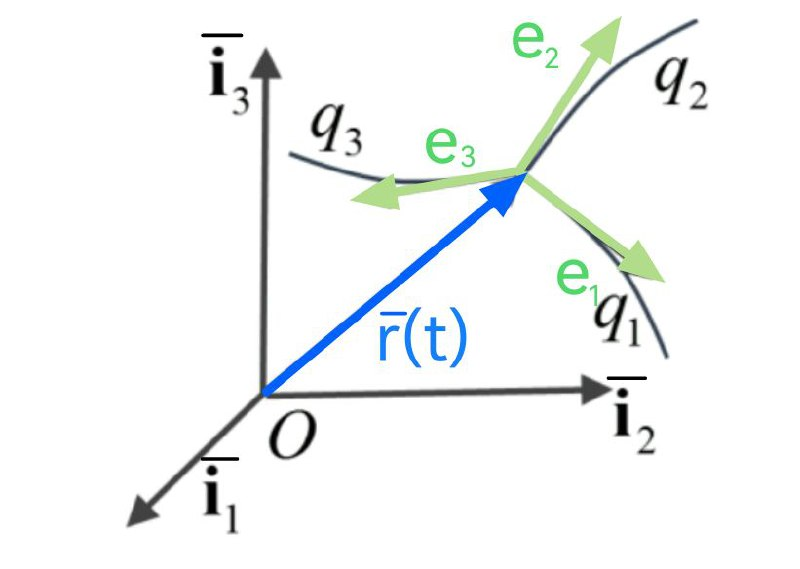
\includegraphics[width=0.8\linewidth]{images/лекция_1_3.jpeg}
\end{wrapfigure}

Рассмотрим материальную точку в криволинейной системе координат $\vec{r} = \vec{r}(q_1,~q_2,`q_3)$. В выбранной точке будем фиксировать пары параметров $q_i$ и $q_j$ и менять третий. Таким образом получим три кривые, по касательным к которым построим локальный базис с ортами
\[
\vec{e_k} = \dfrac{1}{h_k} \cdot \dfrac{\partial \vec{r}}{\partial q_k},
\]
\tab\\ \tab\\ 
где $h_k = |\dfrac{\partial\vec{r}}{\partial q_k} |$ --- \textbf{нормировочный коэффициент Ламе}.\\

\begin{example}
    Рассмотрим цилиндрические координаты:
    \[
    \vec{r} = \begin{pmatrix}
        \rho \cos{\phi}\\
        \rho \sin{\phi}\\
        z\\
    \end{pmatrix}
    \]
    Тогда
    \[
    \vec{e_{\phi}} = \dfrac{1}{h_{\phi}} \cdot \dfrac{\partial \vec{r}}{\partial \phi} \Longrightarrow h_{\phi} = \rho, \ \vec{e_{\phi}} = \begin{pmatrix}
        -\sin{\phi}\\
        \cos{\phi}\\
        0\\
    \end{pmatrix}
    \]
    Аналогично с остальными ортами.
\end{example}

Отсюда найдем скорость материальной точки:
\[
\vec{v} = \dot{\vec{r}}(q_1, q_2, q_3) = \sum\limits_{k = 1}^3{\dfrac{\partial \vec{r}}{\partial q_k} \dot{q}_k} = \sum\limits_{k = 1}^3{h_k\dot{q}_k \cdot \vec{e_k}}
\]
Здесь $h_k q_k$ --- коэффициенты разложения $v$ по локальному базису.\\

Найдем проекции вектора ускорения $w$ на направления локального базиса, т.е. $w_k = \vec{w} \cdot \vec{e_k}$. Для этого рассмотрим
\[
\dfrac{d}{dt}(v \cdot \dfrac{\partial \vec{r}}{\partial q_k}) = \dot{\vec{v}}\cdot \dfrac{\partial \vec{r}}{\partial q_k} + v \dfrac{d}{dt}\dfrac{\partial \vec{r}}{\partial q_k}\eqno{(*)}
\]
\begin{enumerate}
    \item $\dfrac{\partial \vec{r}}{\partial q_k} = \dfrac{\partial \vec{v}}{\partial \dot{q}_k}$, т.к. $\vec{v} = \sum\limits_{k = 1}^3{\dfrac{\partial \vec{r}}{\partial q_k} \dot{q}_k}$
    \item $\dfrac{d}{d t}\dfrac{\partial\vec{r}}{\partial q_k} = \dfrac{\partial\vec{v}}{\partial q_k}$, т.к. $\dfrac{d}{d t}\dfrac{\partial\vec{r}}{\partial q_k} =  \sum\limits_{k = 1}^3{\dfrac{\partial\vec{r}}{\partial q_i \partial q_k} \dot{q_k}} = \dfrac{\partial}{\partial q_k}\sum\dfrac{\partial\vec{r}}{\partial q_i}\dot{q_i} = \dfrac{\partial\vec{v}}{\partial q_k}$
    \item Подставим (1) и (2) в (*).
\end{enumerate}
Итоговая формула
\[
w_k = \dfrac{1}{h_k}\left[\dfrac{d}{d t}\dfrac{\partial(v^2 / 2)}{\partial \dot{q_k}} - \dfrac{\partial(v^2 / 2)}{\partial q_k}\right]
\]